% Options for packages loaded elsewhere
\PassOptionsToPackage{unicode}{hyperref}
\PassOptionsToPackage{hyphens}{url}
%
\documentclass[
  11pt,
  a4paper,
]{article}
\usepackage{amsmath,amssymb}
\usepackage{lmodern}
\usepackage{iftex}
\ifPDFTeX
  \usepackage[T1]{fontenc}
  \usepackage[utf8]{inputenc}
  \usepackage{textcomp} % provide euro and other symbols
\else % if luatex or xetex
  \ifXeTeX
    \usepackage{zxjatype} 
    \usepackage[ipaex]{zxjafont}
  \fi
  \usepackage{unicode-math}
  \defaultfontfeatures{Scale=MatchLowercase}
  \defaultfontfeatures[\rmfamily]{Ligatures=TeX,Scale=1}
\fi
% Use upquote if available, for straight quotes in verbatim environments
\IfFileExists{upquote.sty}{\usepackage{upquote}}{}
\IfFileExists{microtype.sty}{% use microtype if available
  \usepackage[]{microtype}
  \UseMicrotypeSet[protrusion]{basicmath} % disable protrusion for tt fonts
}{}
\usepackage{xcolor}
\IfFileExists{xurl.sty}{\usepackage{xurl}}{} % add URL line breaks if available
\IfFileExists{bookmark.sty}{\usepackage{bookmark}}{\usepackage{hyperref}}
\hypersetup{
  pdftitle={Charitable Giving, Tax Reform, and Self-selection of Tax Report: Evidence from South Korea},
  hidelinks,
  pdfcreator={LaTeX via pandoc}}
\urlstyle{same} % disable monospaced font for URLs
\usepackage[left=3cm,right=3cm,top=3cm,bottom=3cm]{geometry}

\usepackage{setspace}
\renewcommand{\baselinestretch}{1.5}
\usepackage{float}

\usepackage{longtable,booktabs,array}
\usepackage{threeparttable, threeparttablex, multirow}
\usepackage{calc} % for calculating minipage widths
% Correct order of tables after \paragraph or \subparagraph
\usepackage{etoolbox}
\makeatletter
\patchcmd\longtable{\par}{\if@noskipsec\mbox{}\fi\par}{}{}
\makeatother
% Allow footnotes in longtable head/foot
\IfFileExists{footnotehyper.sty}{\usepackage{footnotehyper}}{\usepackage{footnote}}
\makesavenoteenv{longtable}
\usepackage{graphicx}
\makeatletter
\def\maxwidth{\ifdim\Gin@nat@width>\linewidth\linewidth\else\Gin@nat@width\fi}
\def\maxheight{\ifdim\Gin@nat@height>\textheight\textheight\else\Gin@nat@height\fi}
\makeatother
% Scale images if necessary, so that they will not overflow the page
% margins by default, and it is still possible to overwrite the defaults
% using explicit options in \includegraphics[width, height, ...]{}
\setkeys{Gin}{width=\maxwidth,height=\maxheight,keepaspectratio}
% Set default figure placement to htbp
\makeatletter
\def\fps@figure{htbp}
\makeatother
\setlength{\emergencystretch}{3em} % prevent overfull lines
\providecommand{\tightlist}{%
  \setlength{\itemsep}{0pt}\setlength{\parskip}{0pt}}
\setcounter{secnumdepth}{5}
\newlength{\cslhangindent}
\setlength{\cslhangindent}{1.5em}
\newlength{\csllabelwidth}
\setlength{\csllabelwidth}{3em}
\newlength{\cslentryspacingunit} % times entry-spacing
\setlength{\cslentryspacingunit}{\parskip}
\newenvironment{CSLReferences}[2] % #1 hanging-ident, #2 entry spacing
 {% don't indent paragraphs
  \setlength{\parindent}{0pt}
  % turn on hanging indent if param 1 is 1
  \ifodd #1
  \let\oldpar\par
  \def\par{\hangindent=\cslhangindent\oldpar}
  \fi
  % set entry spacing
  \setlength{\parskip}{#2\cslentryspacingunit}
 }%
 {}
\usepackage{calc}
\newcommand{\CSLBlock}[1]{#1\hfill\break}
\newcommand{\CSLLeftMargin}[1]{\parbox[t]{\csllabelwidth}{#1}}
\newcommand{\CSLRightInline}[1]{\parbox[t]{\linewidth - \csllabelwidth}{#1}\break}
\newcommand{\CSLIndent}[1]{\hspace{\cslhangindent}#1}
\ifLuaTeX
  \usepackage{selnolig}  % disable illegal ligatures
\fi

\title{Charitable Giving, Tax Reform, and Self-selection of Tax Report: Evidence from South Korea}


      \usepackage{authblk}
                            \author[]{Hiroki Kato}
                                      \affil{Graduate School of Economics, Osaka University, Japan \thanks{vge008kh@stundent.econ.osaka-u.ac.jp}}
                                                    \author[]{Tsuyoshi Goto}
                                      \affil{Graduate School of Social Sciences, Chiba University, Japan}
                                                    \author[]{Yong-Rok Kim}
                                      \affil{Graduate School of Economics, Kobe University, Japan}
                              
\date{2021/07/26}


\begin{document}
\begin{spacing}{1}
  \maketitle
\end{spacing}
\begin{spacing}{1}
  \begin{abstract}
    This paper investigates (1) the price elasticity of giving and (2) whether the different perception towards the government cause the different giving behavior using South Korean panel data. Our result classifies that the price elasticity of giving in Korea is -0.59 \textasciitilde{} -1.01 for intensive margin and -1.17 \textasciitilde{} -1.48 for extensive margin. We also show that the amount of donation is not different between those who regard government as inefficient and the others, though the giving price elasticity of the former is more elastic than the latter. This means that those who think of government as inefficient have more willingness to donate for 1\% reduction of giving price.
    
            \noindent
    \textbf{Keywords}: Charitable giving, Giving price, Tax reform, South Korea, 
        
        \noindent
    \textbf{JEL Codes}: D91, I10, I18, 
        
  \end{abstract}
\end{spacing}

\hypertarget{introduction}{%
\section{Introduction}\label{introduction}}

In many countries, governments set a tax relief for charitable giving. This is because, if subsidizing charitable giving induces a large increase in donations, it is desirable for public good provision. To evaluate the effect of tax relief, many papers investigate the elasticity of charitable donations with respect to their tax price (Almunia et al., 2020; Auten et al., 2002; Bakija and Heim, 2011; Fack and Landais, 2010; Randolph, 1995). Focusing on the tax deduction or tax credit on the charity, they show that the price elasticity of giving is about -1 or more in terms of absolute value, which means that the tax relief for the charitable giving is good in the sense that 1\% tax relief derives more than 1\% donation.

However, if the government can provide public good more efficiently than the direct donation, the donation may not be preferable because the public good provision via donation would be costly then.
Moreover, when the government is much more efficient than charities, people may not donate so much even if they have a warm-glow preference. Saez (2004) suggests that the change of the relative price between public good provision by donation and government will change the behavior of people and the price elasticity of donation.
However, the evaluation about the efficiency of the government is usually subjective and different for people. If someones regard the government as efficient, the perceived relative price of giving would be high for them. Thus, the giving behavior would be affected by the subjective perception towards the government.

Considering these points, this paper investigates (1) the price elasticity of giving and (2) whether the different perception towards the government cause the different giving behavior using South Korean panel data.
Our first main concern is the price elasticity of charity. South Korea (Korea hereafter) experienced the tax reform in 2014, from when the tax relief on charitable giving was conducted by tax credit, though tax deduction had been used before 2014. Thus, we exploit this tax reform as an exogenous policy change to derive the price elasticity of giving. Since the extant research focus on the tax reform within the scheme of tax deduction or tax credit, this paper firstly deals with the tax reform from tax deduction system to tax credit system.
Our result classifies that the price elasticity of giving in Korea is -0.59 \textasciitilde{} -1.01 for intensive margin and -1.17 \textasciitilde{} -1.48 for extensive margin.

Our second concern is the relationship between the giving behavior and the perception towards the government. As we explained, people feeling administrative inefficiency would consider the direct donation is more efficient and would have more willingness to donate. Using the Korean field data, we investigate this and show that the giving price elasticity of those who regard government as inefficient is more elastic than the others. This means that those who think of government as inefficient have more willingness to donate for 1\% reduction of giving price.

This paper contributes two strands of charitable giving literature: the elasticity of charitable donations with respect to their tax price and the perception of government's inefficiency. The examples of papers in the first strand are Randolph (1995), Auten et al. (2002), Fack and Landais (2010), Bakija and Heim (2011), and Almunia et al. (2020). They typically use the tax return data, the main part of which is the data about wealthy people. Since our data is based on survey, which reflects the income distribution of population, we believe that we can estimate the giving price elasticity of population more precisely. Using the data with low-income households may be difficult to estimate the giving price elasticity in terms of intensive margin since they are expected to donate less than high-income households. To address this issue, we estimate not only the elasticity of intensive margin, as most of papers do, but also the elasticity of extensive margin following Almunia et al. (2020).
Moreover, we use the data of Korea, a non-Western country, which the extant research did not examine.\footnote{This point may be important since Kim (2021) reports that the giving behavior is strongly affected by the cultural matter such as the religious belief.}

In the second strand, there are some experimental studies and papers considering the tax evasion. Using an experiment, Li et al. (2011) compare people's willingness to give money for private charities and government agencies whose missions are the same. They show that people tend to donate for private charities more than government agency though they do not directly investigate the relationship between people's perception toward the government and giving behavior. Sheremeta and Uler (2020) show that people increase the voluntary public good provision when they face the wasteful government spending in the experimental setting. Although the government in their setting does not provide public good, they suggest that the willingness for donation may increase if people perceive the inefficiency of government. In the tax evasion literature, several paper suggests the perceived inefficiency of government reduce tax morale (Anderson, 2017; Frey and Torgler, 2007; Hammar et al., 2009). We contribute on this literature by showing the relation between the perception of government efficiency and the giving behavior.

This paper consist of seven sections. Section 2 and 3 respectively explain the institutional background and data. Section 4 explains the estimation method. Section 5 deals with the analysis of giving price elasticity and section 6 shows the analysis of perceptions toward the government. Section 7 concludes.

\hypertarget{institutional-background}{%
\section{Institutional background}\label{institutional-background}}

In this section, we describe the income tax relief for charitable giving in Korea and used dataset.

\hypertarget{tax-relief-for-charitable-giving-by-tax-deduction-and-tax-credit}{%
\subsection{Tax relief for charitable giving by tax deduction and tax credit}\label{tax-relief-for-charitable-giving-by-tax-deduction-and-tax-credit}}

In the South Korea, the tax policy about charitable giving drastically changed in 2014. Before then, tax relief of charitable giving was provided by tax deduction while, from 2014, tax relief by tax credit was introduced instead of tax deduction.

The tax deduction and tax credit may have different effects on giving behavior. This subsection summarize the difference of tax deduction and tax credit.
Consider that a household has a choice between private consumptions (\(x_i\)) and charitable giving (\(g_i\)). Let \(y_i\) be pre-tax total income.
Then, the budget constraint is

\[
    x_i + g_i = y_i - T_i(y_i, g_i).
\]
\(T_i\) is tax amount which depends on the pre-tax income and charitable giving.
On one hand, tax deduction reduces taxable income by giving. The amount of tax is

\[
    T_i = \tau(y_i - g_i) \cdot (y_i - g_i),
\]

where \(\tau(\cdot)\) is the income tax rate which is determined by \(y_i - g_i\).\footnote{\(\tau(\cdot)\) here is a function which shows the average tax rate, which is determined progressively. Since the price elasticity of giving shows the marginal and additional increment for one unit of price reduction increase, we use not average but marginal tax rate to construct the giving price following the literature. Usage of the function of the average tax rate here is for explanatory simplicity.} The budget constraint will be

\[
    x_i + [1 - \tau(y_i - g_i)]g_i = [1 - \tau(y_i - g_i)] y_i.
\]

Thus, the giving price compared to the price of private consumption is \(p_i^{d} \equiv 1 - \tau(y_i - g_i)\) in tax deduction system. Since the giving price in tax deduction scheme varies depending on (1) the income level and (2) the amount of charitable giving, it is endogenous to them, i.e.~(1) and (2).

On the other hand, tax credit reduces tax amount directly, that is,

\[
    T_i = \tau(y_i)\cdot y_i - m g_i,
\]

where \(m \in [0, 1]\) is the tax credit rate. Under the tax credit system, the budget constraint is

\[
    x_i + (1 - m) g_i = [1 - \tau(y_i)] y_i.
\]

Thus, the giving price of tax credit system will be \(p_i^c = 1 - m\), which is only dependent on the tax credit rate \(m\), which is exogenously determined by the government.
Therefore, the giving price in the tax credit system would not be manipulated by donors.

\begin{table}

\caption{\label{tab:tabTaxRate}Marginal Income Tax Rate}
\centering
\fontsize{7}{9}\selectfont
\begin{threeparttable}
\begin{tabular}[t]{lccccccc}
\toprule
Income/Year & 2008 & 2009 & 2010 \textasciitilde{} 2011 & 2012 \textasciitilde{} 2013 & 2014 \textasciitilde{} 2016 & 2017 & 2018\\
\midrule
(A) \textasciitilde{} 1200 & 8\% & 6\% & 6\% & 6\% & 6\% & 6\% & 6\%\\
\cmidrule{1-8}
(B) 1200 \textasciitilde{} 4600 & 17\% & 16\% & 15\% & 15\% & 15\% & 15\% & 15\%\\
\cmidrule{1-8}
(C) 4600 \textasciitilde{} 8800 & 26\% & 25\% & 24\% & 24\% & 24\% & 24\% & 24\%\\
\cmidrule{1-8}
(D) 8800 \textasciitilde{} 15000 &  &  &  &  & 35\% &  & 35\%\\
\cmidrule{1-1}
\cmidrule{6-6}
\cmidrule{8-8}
(E) 15000 \textasciitilde{} 30000 &  &  &  & \multirow{-2}{*}{\centering\arraybackslash 35\%} &  & \multirow{-2}{*}{\centering\arraybackslash 35\%} & 38\%\\
\cmidrule{1-1}
\cmidrule{5-5}
\cmidrule{7-8}
(F) 30000 \textasciitilde{} 50000 &  &  &  &  &  & 38\% & 40\%\\
\cmidrule{1-1}
\cmidrule{7-8}
(G) 50000 \textasciitilde{} & \multirow{-4}{*}{\centering\arraybackslash 35\%} & \multirow{-4}{*}{\centering\arraybackslash 35\%} & \multirow{-4}{*}{\centering\arraybackslash 35\%} & \multirow{-2}{*}{\centering\arraybackslash 38\%} & \multirow{-3}{*}{\centering\arraybackslash 38\%} & 40\% & 42\%\\
\bottomrule
\end{tabular}
\begin{tablenotes}
\item Notes: Marginal income tax rates applied from 2008 to 2018 are summarized. The income level is shown in terms of 10,000 KRW, which is approximately 10 United States dollars (USD) at an exchange rate of 1,000 KRW to one USD.
\end{tablenotes}
\end{threeparttable}
\end{table}

\hypertarget{our-identification-strategy}{%
\subsection{Our Identification Strategy}\label{our-identification-strategy}}

In 2014, aiming at the relaxation of regressivity of giving price, the Korean government reformed tax system again, where the tax credit was introduced instead of tax deduction. Since then, 15\% of the total amount of charitable giving has been allowed as a tax credit, which means that the giving price from 2014 is 0.85 irrelevant to the income level.

Summarizing this, compared to tax credit system, the high income household, whose (average) income tax rate is more than 15\%, get benefit from charitable giving under the tax deduction system. However, middle or low income households would enjoy tax relief in tax credit system more than tax deduction system. We exploit this policy change as an identification strategy.

\hypertarget{korean-tax-reform-in-2014}{%
\subsection{Korean tax reform in 2014}\label{korean-tax-reform-in-2014}}

The tax incentives for charitable giving in Korea stared in 1967 and the market of charitable giving in Korea totaled 10.9 trillion KRW (approximately 1.09 bilion USD, 0.761\% of GDP) in 2012 according to the national tax statistics.
Since the income tax deduction was initially used as a tax incentive and the marginal income tax rate was determined as Table \ref{tab:tabTaxRate}, the minimum giving price before 2014 was 0.62.

In 2014, aiming at the relaxation of regressivity of giving price, the Korean government reformed tax system again, where the tax credit was introduced instead of tax deduction. Since then, 15\% of the total amount of charitable giving has been allowed as a tax credit, which means that the giving price from 2014 is 0.85 irrelevant to the income level.

Summarizing this, compared to tax credit system, the high income household, whose (average) income tax rate is more than 15\%, get benefit from charitable giving under the tax deduction system. However, middle or low income households would enjoy tax relief in tax credit system more than tax deduction system. We exploit this policy change as an identification strategy.

\hypertarget{data}{%
\section{Data}\label{data}}

The National Survey of Tax and Benefit (hereafter, NaSTab) is an annual financial panel survey
implemented by The Korea Institute of Taxation and Finance
to study the tax burden of households and the benefits that households receive from the government.
The subjects of this survey are general households and household members living in 15 cities and provinces nationwide.
This survey is based on a face-to-face interview.\footnote{If it is difficult for investigators to meet subjects, another family member answers on behalf of him.}
The NaSTaB data is constructed as the subjects represent the population of Korean society.
This enables us to derive giving price elasticity of population without re-weighting samples, which is used in the extant research.
Moreover, note that subjects are not limited to the taxpayer or income earner reflecting the population.
We use this panel survey from 2013 to 2019 because we focus on the 2014 tax reform.
In addition, we exclude the subject of the sample, whose age is under 23, since they are not likely to have income or assets.

\begin{table}

\caption{\label{tab:SummaryCovariate}Descriptive Statistics}
\centering
\fontsize{7}{9}\selectfont
\begin{tabular}[t]{lcccccc}
\toprule
 & N & Mean & Std.Dev. & Min & Median & Max\\
\midrule
\addlinespace[0.3em]
\multicolumn{7}{l}{\textbf{Charitable Donations}}\\
\hspace{1em}Annual charitable giving (unit: 10,000KRW) & 67848 & 29.52 & 132.91 & 0.00 & 0.00 & 10000.00\\
\hspace{1em}Dummy of Donation > 0 & 67848 & 0.20 & 0.40 & 0.00 & 0.00 & 1.00\\
\addlinespace[0.3em]
\multicolumn{7}{l}{\textbf{Income, giving price, and tax report}}\\
\hspace{1em}Annual taxable labor income (unit: 10,000KRW) & 53269 & 1876.12 & 2700.97 & 0.00 & 900.00 & 91772.00\\
\hspace{1em}First giving price & 62877 & 0.86 & 0.04 & 0.62 & 0.85 & 0.94\\
\hspace{1em}Dummy of tax report of charitable giving & 12172 & 0.48 & 0.50 & 0.00 & 0.00 & 1.00\\
\addlinespace[0.3em]
\multicolumn{7}{l}{\textbf{Individual Characteristics}}\\
\hspace{1em}Age & 67848 & 51.35 & 15.81 & 24.00 & 50.00 & 104.00\\
\hspace{1em}Female dummy & 67848 & 0.53 & 0.50 & 0.00 & 1.00 & 1.00\\
\hspace{1em}Employee dummy & 42362 & 0.53 & 0.50 & 0.00 & 1.00 & 1.00\\
\hspace{1em}University graduate & 67842 & 0.41 & 0.49 & 0.00 & 0.00 & 1.00\\
\hspace{1em}High school graduate dummy & 67842 & 0.35 & 0.48 & 0.00 & 0.00 & 1.00\\
\hspace{1em}Junior high school graduate dummy & 67842 & 0.24 & 0.43 & 0.00 & 0.00 & 1.00\\
\bottomrule
\end{tabular}
\end{table}

Table \ref{tab:SummaryCovariate} shows summary statistics of our data.\footnote{Respondents answer the amount of donation for seven specific purposes last year. Seven specific purposes are policitical parties, educational organizations, social welfare organizations, organizations for culutre and art, religious groups, charity activies organaized by religious group, other purposes. We sum up the amount of donations, and consider it as the annual charitable giving.}
The first panel of this table shows variables about charitable giving.
The NaSTaB asks respondents to answer the amount of donation last year.
This is the first outcome variables.
Using this, we make a dummy taking 1 if respondent donated last year.
This is the second outcome variables to estimate the price effect on the decision of donations (extensive margin).
Table \ref{tab:SummaryCovariate} shows that
the average amount of donation is almost 300,000 KRW,
and the proportion of donors is roughly 20\%.
Figure \ref{fig:SummaryOutcome} shows the time-series of two variables.
The blue line shows the average amount of donation among donors.
In each year, its value is nearly 1.5 million KRW,
which is 7\% of average annual taxable income.
The grey bar shows the proportion of donors.
After the tax reform, the proportion of donors decreases by 2\%.
After that, the proportion of donors is greter than 20\%.

\begin{figure}[t]

{\centering 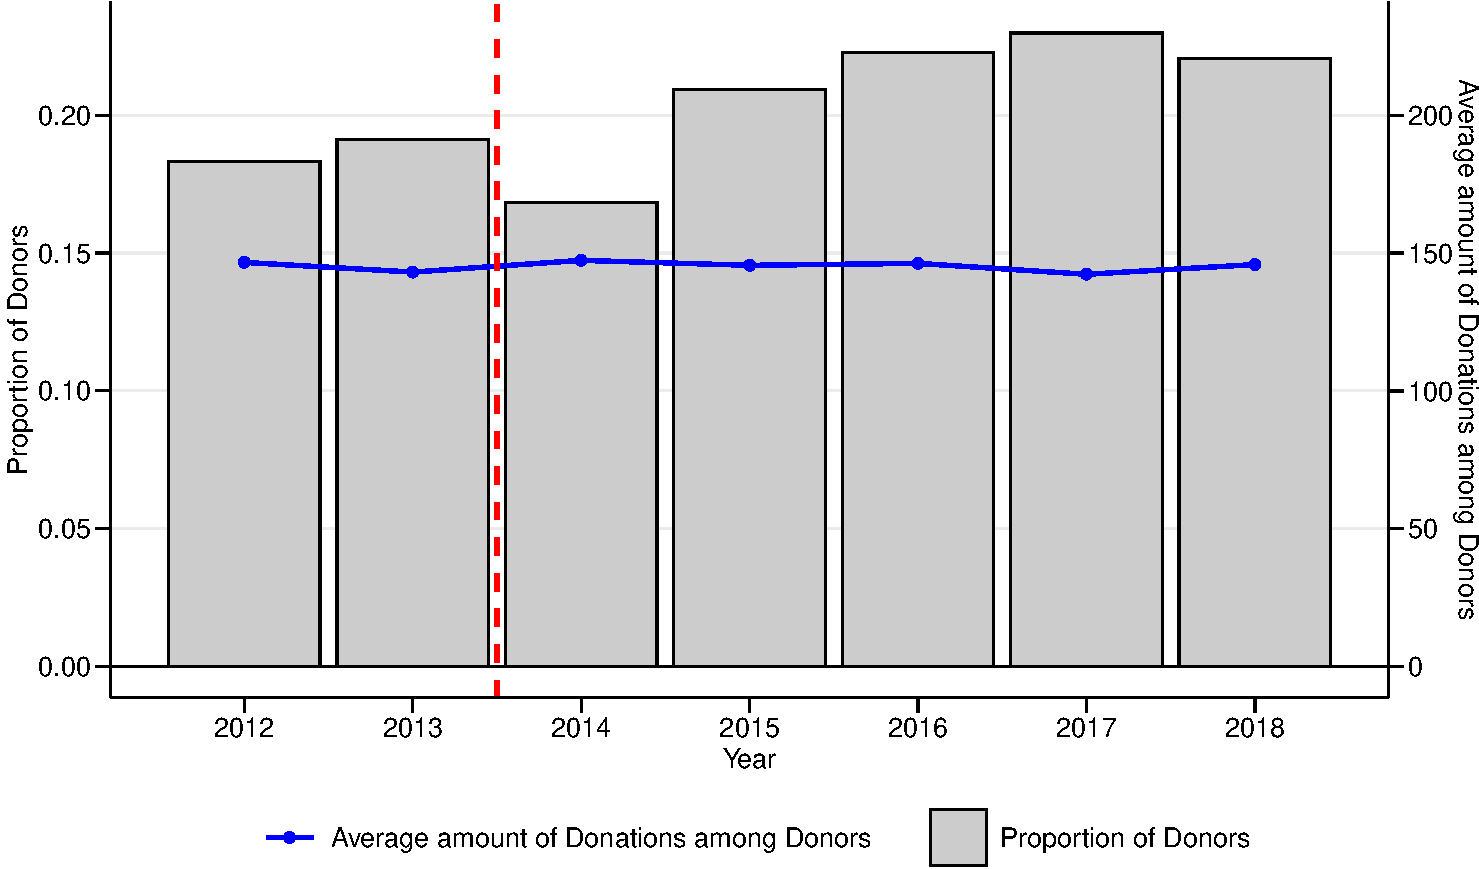
\includegraphics[width=1\linewidth]{C:/Users/katoo/Desktop/NASTAB/paper/draft_files/figure-latex/SummaryOutcome-1} 

}

\caption{Proportion of Donors and Average Donations among Donors. Notes: The left and right axises respectively mesure proportion of donors and the average amount donations among donors. Authors made this graph based on NasTaB data.}\label{fig:SummaryOutcome}
\end{figure}

The second panel of Table \ref{tab:SummaryCovariate} shows variables about income, tax report, and the giving price.
NaSTaB asks respondents to answer the annual labor income last year.
In our sample, the average annual taxable income is 18.76 million KRW.
According to the National Tax Statistical Yearbook published by Korean National Tax Service,
the average annual taxable income is 32.77 million from 2012 to 2018
for employees who submitted the tax return.
Since our sample includes subjects with no labor income, such as housewives,
our sample mean of income is lower than the average income calculated by the public organizations.
In Figure \ref{fig:SummaryPriceChange},
the grey bars show the distribution of annual taxable income in 2013.
The income distribution is left-skewed.

Using this variable, we construct the giving price under the tax deduction system (2012 and 2013).\footnote{The giving price shown in Table \ref{tab:SummaryCovariate} is the \emph{first} giving price. The giving price can be manipulated by an amount of donation. To avoid this endogeneity, we use the giving price where the amount of donation is zero. We will discuss this issue in the next section.}
After the tax reform (after 2014), the giving price is 0.85 regardless of labor income.
as we explained in the section \ref{institutional-background}.
In Figure \ref{fig:SummaryPriceChange},
the blue line shows the giving price in 2012 and 2013,
while the red dashed line shows the giving price after 2014.
From this figure,
those whose annual income is less than 120,000,000 KRW in 2013 could receive benefit from the 2014 tax reform
because the tax reform decreases the giving price.
On the other hand,
those whose annual income is greater than 460,000,000 KRW in 2013 had a loss by the 2014 tax reform
since the tax reform increases the giving price.

The NaSTaB also asks respondents to answer whether they applied for a tax deduction of giving.
Although this variable is unique, the sample size is relatively small due to unanswering.
This survey investigates separately for the case of \emph{total} income (for example, business income, dividend income, rental income)
and the case of \emph{labor} income.
We make a dummy taking one if respondents applied for a business income deduction of giving
or a labor income deduction of giving.
Table \ref{tab:SummaryCovariate} shows the proportion of tax deduction is about 48\%.

\begin{figure}[t]

{\centering 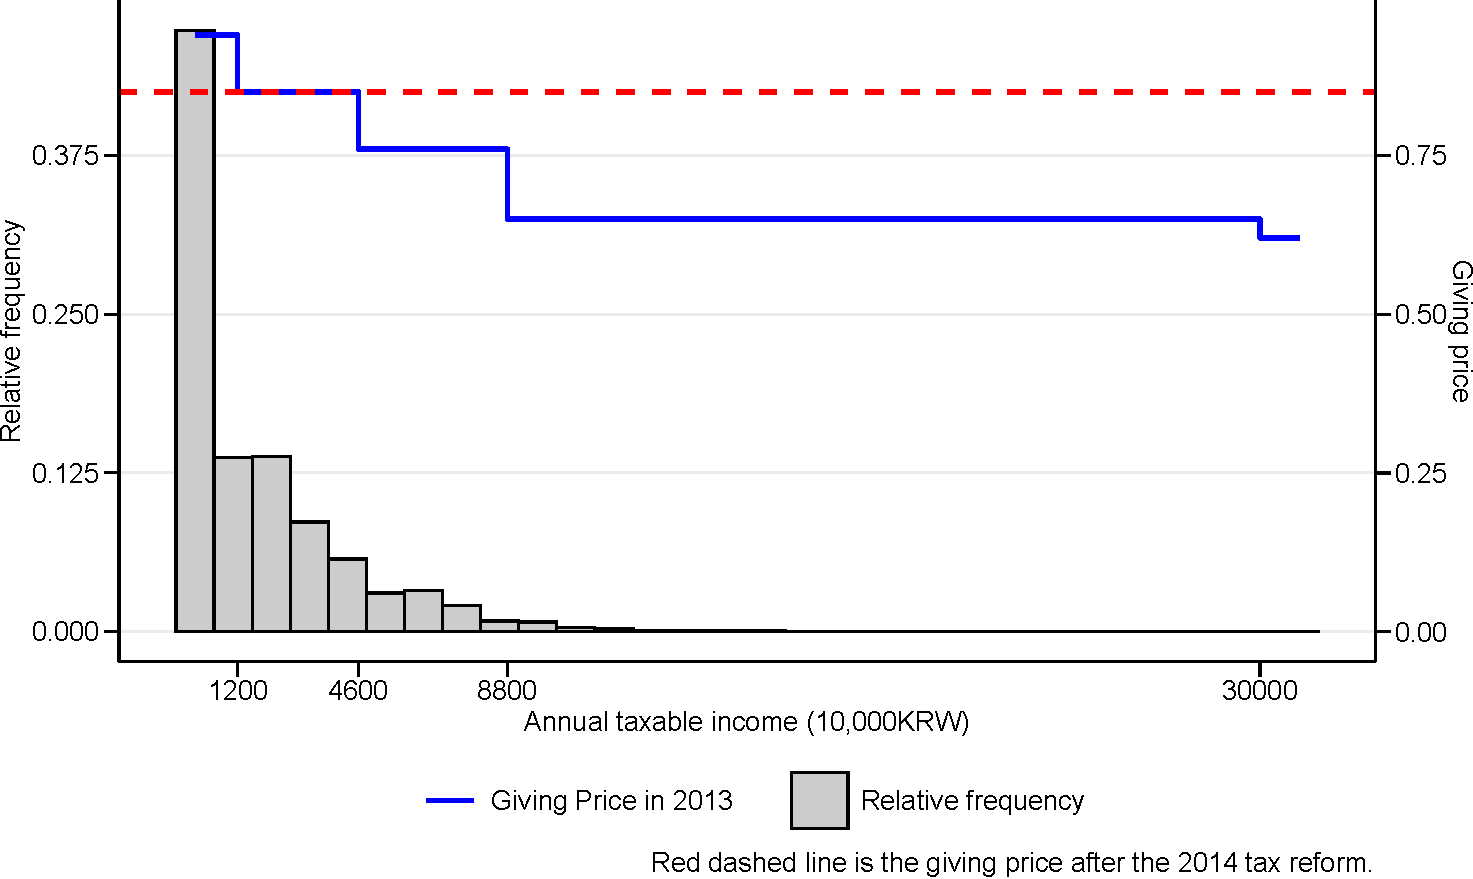
\includegraphics[width=0.9\linewidth]{C:/Users/katoo/Desktop/NASTAB/paper/draft_files/figure-latex/SummaryPriceChange-1} 

}

\caption{Income Distribution and Giving Price in 2013}\label{fig:SummaryPriceChange}
\end{figure}

\hypertarget{estimation}{%
\section{Estimation}\label{estimation}}

Following Almunia et al. (2020), we estimate giving price elasticity for intensive margin and extensive margin. The elasticity of intensive margin shows how much donors additionally donates reacting to the marginal increase of giving price, while the elasticity of extensive margin shows how much the probability to donate changes reacting to marginal increase of giving price. We estimate the elasticity of intensive margin using the following specification:

\begin{equation}
    \ln g_{it} = \varepsilon^{int}_p R_{it} \ln p_{it} + \varepsilon^{int}_y \ln y_{it} 
    + X_{it}\beta +\mu_i +\iota_t +u_{it}. \label{eq:intensive}
\end{equation}

\(g_{it}, p_{it}\) and \(y_{it}\) respectively indicates the amount of giving, the giving price, and income of \(i\) in year \(t\).
\(R_{it}\) is a dummy taking one if individual \(i\) applied for a tax deduction in year \(t\).
\(\mu_i, \iota_t\) and \(u_{it}\) are individual fixed effect, year fixed effect and error term, respectively.
The individual fixed effect controls for time-invariant individual characteristics. The year fixed effect controls for events that affect all subjects at the same time. \(X_{it}\) is a vector of covariates which include variables about education and gender. Moreover, we add some interaction terms between year fixed effect and control variables into \(X_{it}\), since they will control for events that affects subject with specific characteristics at the same time following Zeldow and Hatfield (2019).

On the other hand,
the elasticity of extensive margin is estimated using the linear probability model such as

\begin{equation}
D_{it} =  \delta R_{it} \ln p_{it} +\gamma \ln y_{it} + X_{it}\beta +\mu_i  +\iota_t +v_{it}. \label{eq:extensive}
\end{equation}

\(D_{it}\) is a dummy variable taking 1 if individual \(i\) donates at year \(t\) and 0 otherwise.
Since we use the linear probability model,
the estimated coefficient \(\delta\) represents \(\hat{\delta} = \frac{\partial D_{it}}{\partial p_{it}} p_{it}\).
Also, the estimated coefficient \(\gamma\) represents \(\hat{\gamma} = \frac{\partial D_{it}}{\partial y_{it}} y_{it}\).
Thus, the implied extensive-margin price and income elasticity are obtained by
\(\hat{\delta}/\bar{D}\) and \(\hat{\gamma}/\bar{D}\), respectively,
where \(\bar{D}\) is sample average of outcome variable \(D_{it}\).

As shown in the section \ref{institutional-background},
the giving price \(p_{it}\) is defined as follows:

\begin{align}
  p_{it}(y_{it}, g_{it}) =
  \begin{cases}
    1 - \tau_t(y_{it} - g_{it})  \quad\text{if}\quad t < 2014  \\
    1 - m \quad\text{if}\quad t \ge 2014
  \end{cases}, \label{eq:price}
\end{align}
where \(\tau_t(\cdot)\) is average tax rate in year \(t\).

Our identification assumption is that the \emph{within} price variation is exogenous due to the fixed effect model.
From the equation \eqref{eq:price},
the within price variation comes from the 2014 tax reform, the within variation of giving \(g_{it}\) and income \(y_{it}\).
Moreover, by the equation \eqref{eq:intensive} and \eqref{eq:extensive},
the within price variation comes from tax report \(R_{it}\).
Since these three variables are self-selected,
we need to solve three potential endogeneity problem to hold our identification assumption.

As a benchmark, we estimate the equation \eqref{eq:intensive} and \eqref{eq:extensive},
assuming that \(R_{it} = 1\) for all \(i\).
This means that we see individuals who did not apply for a tax deduction as those who applied for a tax deduction.
In the treatment effect literature, this effect is sometimes called ``intention-to-treat'' effect (ITT).
By this assumption,
we can solve the issue that the self-selection of tax deduction (\(R_{it}\)) affects the giving price.
Later, we relax this assumption, using the instrumental variable strategy.

Next, we deal with the the possibility that the giving price is endogenous because
the tax payer can reduce their giving price by reducing their amount of donation
and shifting themselves to the lower tax bracket in the tax deduction system (self-selection of \(g_{it}\)).
Since this issue does not happen for the first one unit of donation, whose price (``first price'') cannot be changed by adjusting the donation, we use this first price as the giving price in the estimation.
The first price is obtained by \(p^f_{it} = p_{it}(y_{it}, g_{it})\) evalueated at \(g_{it} = 0\).
As long as income \(y_{it}\) is exogenous, the within giving price \(p^f_{it}\) is also exogenous.
Thus, assuming income \(y_{it}\) is exogenous variable,
we first estimate the first-price elasticity with the equation \eqref{eq:intensive} and \eqref{eq:extensive}
which replace \(\ln p_{it}\) with \(\ln p^f_{it}\).
Moreover, we also estimate the last-price elasticity, using the first price \(p^f_{it}\) as an instrument.

We can justify the first price method, assuming that income is exogenous.
The second approach relaxes this assumption.
Under the tax deduction system,
the change of income have effects on both donations through the income effect
and the giving price through the marginal tax rate.
Therefore,
we employ lagged values of taxable income and
construct a variable for the change in the first price of giving as following:

\[
\ln \left(\frac{p_{it}(y_{it-k} - g_{it-k})}{p_{it-k}(y_{it-k} - g_{it-k})}\right).
\]

where \(g_{it-k} = 0\).
The numerator is the first price that individual \(i\) would have faced in year \(t\)
if she had declared her year \((t - k)\) taxable income at that year.
By fixing the income at year \(t - k\), the instrument isolates changes in price from income responses to the tax reform.
Note that this problem does not happen for the tax credit system, where the giving price is the same across all individuals.

\hypertarget{main-results}{%
\section{Main Results}\label{main-results}}

\hypertarget{price-and-income-elasticity}{%
\subsection{Price and Income Elasticity}\label{price-and-income-elasticity}}

Before the estimation of giving price elasticities for intensive and extensive margin, we estimate the elasticity without distinguishing them. We call this elasticity as overall elasticity.
Table \ref{tab:MainOverall} shows estimation results of overall elasticity.
The column (1) is the baseline estimation, which include individual and time fixed effects.
The price elasticity is rougly -1, which is statistically significant different from zero.
This implies that 1\% increase of giving price raise charitable giving by 1\%.
This result is in line with previous researches which focus on Western countries.
The income elasticity is about 5.3, which is statistically significant different from zero.
This implies that 1\% increase of annual income raise charitable giving by 5.3\%.
The remaining four columns control for events that affects subject with specific characteristics at the same time.
As a result, the price elasticity is more elastic than the baseline result.
The price elasticity lies between -1.3 and -1.1.
On the other hand, the income elasticity is less elastic than the baseline result.
The income elasticity lies between -5.1 and -4.9.

\begin{table}

\caption{\label{tab:MainOverall}Main Results: Overall Elasticity of First Price}
\centering
\fontsize{7}{9}\selectfont
\begin{threeparttable}
\begin{tabular}[t]{lccccc}
\toprule
 & (1) & (2) & (3) & (4) & (5)\\
\midrule
ln(giving price) & -1.072*** & -1.264*** & -1.291*** & -1.114*** & -1.241***\\
 & (0.202) & (0.213) & (0.230) & (0.229) & (0.227)\\
ln(annual taxable income) & 5.393*** & 5.080*** & 5.047*** & 5.116*** & 4.946***\\
 & (0.970) & (0.964) & (0.964) & (0.966) & (0.949)\\
Individual FE & Y & Y & Y & Y & Y\\
Time FE & Y & Y & Y & Y & Y\\
Age & N & Y & Y & Y & Y\\
Year x Education & N & N & Y & Y & Y\\
Year x Gender & N & N & N & Y & Y\\
Year x Resident Area & N & N & N & N & Y\\
N & 53269 & 53269 & 53267 & 53267 & 53267\\
Adjusted R-squared & 0.526 & 0.526 & 0.526 & 0.527 & 0.530\\
\bottomrule
\end{tabular}
\begin{tablenotes}
\item Notes: $^{*}$ $p < 0.1$, $^{**}$ $p < 0.05$, $^{***}$ $p < 0.01$. Standard errors are clustered at individual level. When controlling age, we alson include its squared term.
\end{tablenotes}
\end{threeparttable}
\end{table}

Table \ref{tab:MainIntensive} shows the intensive-margin and the extensive-margin elasticities.
The first panel shows the intensive-margin elasticity.
Compared to the overall elasticitiy, the price and income elasticitiy are less elastic.
Controlling individual and time fixed effects,
the price and income elasticity is about -0.6 and about 2,
which are statistically significant different from zero (See the column (1)).
Moreover, when we include the interaction term between individual characteristics and year dummies,
these values vary.
The price elasticity lies between -1.1 and -0.8,
and the income elasticity lies between 1.4 and 1.6.
Anyway, our conlusion is that the amount of donations is insensitive to the giving price among donors.

\begin{table}

\caption{\label{tab:MainIntensive}Main Results: Intensive-Margin Elasticity of First Price}
\centering
\fontsize{7}{9}\selectfont
\begin{threeparttable}
\begin{tabular}[t]{lccccc}
\toprule
 & (1) & (2) & (3) & (4) & (5)\\
\midrule
ln(giving price) & -0.593*** & -0.838*** & -1.016*** & -0.893*** & -0.904***\\
 & (0.203) & (0.212) & (0.232) & (0.243) & (0.249)\\
ln(annual taxable income) & 2.015*** & 1.562** & 1.445** & 1.528** & 1.571**\\
 & (0.675) & (0.655) & (0.647) & (0.651) & (0.653)\\
Individual FE & Y & Y & Y & Y & Y\\
Time FE & Y & Y & Y & Y & Y\\
Age & N & Y & Y & Y & Y\\
Year x Education & N & N & Y & Y & Y\\
Year x Gender & N & N & N & Y & Y\\
Year x Resident Area & N & N & N & N & Y\\
N & 11637 & 11637 & 11637 & 11637 & 11637\\
Adjusted R-squared & 0.675 & 0.675 & 0.676 & 0.676 & 0.678\\
\bottomrule
\end{tabular}
\begin{tablenotes}
\item Notes: $^{*}$ $p < 0.1$, $^{**}$ $p < 0.05$, $^{***}$ $p < 0.01$. Standard errors are clustered at individual level. When controlling age, we alson include its squared term.
\end{tablenotes}
\end{threeparttable}
\end{table}

Table \ref{tab:MainExtensive} shows the extensive-margin elasticity.
By results of overall elasticities and the intensive-margin elasticities,
we expect that the extensive-margin price and income elasticity is more elastic than the overall elasticities.
In the column (1), the coefficient of logged giving price and logged annual income are -0.257 and 1.175 respectively,
which are statistically significant different from zero.
Since we use the linear probability model,
we need to calculate \(\epsilon^p_{EXT} = -0.257/D_{it}\) and \(\epsilon^y_{EXT} = 1.175/D_{it}\)
to obtain the price and income elasticity, respectively.
Especially, the coefficient of logged giving price represents the lower-bound of price elasticity
because the variable \(D_{it}\) takes either 0 or 1.
When we evaluate the price elasticity at the sample mean of \(D_{it}\),
the implied price elasticity is -1.264, which is slightly more elastic than the overall one.
Also, we evaluate the income elasticity at the sample mean of outcome.
The implied income elasticity is 5.778, which is slightly more elastic than the overall one.
Although the implied price and income elasticity varies with covariates,
results are in line with our expectation.
Thus, the decision of donations is sensitive to the giving price and annual income.

\begin{table}

\caption{\label{tab:MainExtensive}Main Results: Extensive-Margin Elasticity of First Price}
\centering
\fontsize{7}{9}\selectfont
\begin{threeparttable}
\begin{tabular}[t]{lccccc}
\toprule
 & (1) & (2) & (3) & (4) & (5)\\
\midrule
ln(giving price) & -0.257*** & -0.288*** & -0.273*** & -0.237*** & -0.267***\\
 & (0.046) & (0.048) & (0.052) & (0.052) & (0.051)\\
ln(annual taxable income) & 1.175*** & 1.124*** & 1.125*** & 1.139*** & 1.102***\\
 & (0.223) & (0.223) & (0.223) & (0.224) & (0.220)\\
 &  &  &  &  & \\
Implied price elasticity & -1.176*** & -1.320*** & -1.250*** & -1.086*** & -1.221***\\
 & (0.210) & (0.221) & (0.239) & (0.238) & (0.235)\\
Implied income elasticity & 5.379*** & 5.145*** & 5.148*** & 5.212*** & 5.045***\\
 & (1.023) & (1.021) & (1.023) & (1.024) & (1.005)\\
Individual FE & Y & Y & Y & Y & Y\\
Time FE & Y & Y & Y & Y & Y\\
Age & N & Y & Y & Y & Y\\
Year x Education & N & N & Y & Y & Y\\
Year x Gender & N & N & N & Y & Y\\
Year x Resident Area & N & N & N & N & Y\\
N & 53269 & 53269 & 53267 & 53267 & 53267\\
Adjusted R-squared & 0.458 & 0.458 & 0.458 & 0.458 & 0.462\\
\bottomrule
\end{tabular}
\begin{tablenotes}
\item Notes: $^{*}$ $p < 0.1$, $^{**}$ $p < 0.05$, $^{***}$ $p < 0.01$. Standard errors are clustered at individual level. When controlling age, we alson include its squared term. The implied extensive-marign price elasticity is evaluated at the sample mean of $D_{ijt}$.
\end{tablenotes}
\end{threeparttable}
\end{table}

In summary, our first conclusion is that
the decision of donations is sensitive to the giving price,
and the amount of donations is insensitive to the giving price once they decide to donate.
In the next subsection, we check the robustness of our first conclusion, using three methods.

\hypertarget{robustness-check}{%
\subsection{Robustness Check}\label{robustness-check}}

The first robustness check estimates the last price elasticity using the first price of giving as an instrument.
Our main results show that \emph{first} price elasticity to avoid the endogeneity of giving price.
However, the first price elasiticity is not realistic
because people face the \emph{last} marginal price when deciding amount of donations.
Thus, we estimate the \emph{last} price elasticity, using the Panel IV method.

There is one caution to interpret the last price elasticity.
Under the tax credit system, the last price elasticity is equivalent to the first one.
Since major observation units are observed when the tax credit system is implemented,
the last giving price is strongly correlated with the first one.
In other words, covariates between the last and first giving price is roughly equal to one.
In the first stage, the coefficient of first giving price is roughly 0.98 in any specifications.\footnote{We do not show the first-stage results. Instead, we show the F-statistics of the instrument variable.}
Thus, our last price elasticity may be upper bound of true price elasticity.

\begin{table}

\caption{\label{tab:LastOverall}Overall Elasticity of Last Price}
\centering
\fontsize{7}{9}\selectfont
\begin{threeparttable}
\begin{tabular}[t]{lccccc}
\toprule
 & (1) & (2) & (3) & (4) & (5)\\
\midrule
ln(last giving price) & -2.421*** & -2.536*** & -2.750*** & -2.529*** & -2.650***\\
 & (0.204) & (0.216) & (0.233) & (0.231) & (0.229)\\
ln(annual taxable income) & 5.258*** & 5.072*** & 4.981*** & 5.058*** & 4.910***\\
 & (0.961) & (0.961) & (0.959) & (0.961) & (0.948)\\
Individual FE & Y & Y & Y & Y & Y\\
Time FE & Y & Y & Y & Y & Y\\
Age & N & Y & Y & Y & Y\\
Year x Education & N & N & Y & Y & Y\\
Year x Gender & N & N & N & Y & Y\\
Year x Resident Area & N & N & N & N & Y\\
N & 52304 & 52304 & 52302 & 52302 & 52302\\
Adjusted R-squared & 0.529 & 0.529 & 0.529 & 0.530 & 0.533\\
\bottomrule
\end{tabular}
\begin{tablenotes}
\item Notes: $^{*}$ $p < 0.1$, $^{**}$ $p < 0.05$, $^{***}$ $p < 0.01$. Standard errors are clustered at individual level. The instumental variable is the first giving price in year $t$. When controlling age, we alson include its squared term.
\end{tablenotes}
\end{threeparttable}
\end{table}

\begin{table}

\caption{\label{tab:LastIntensive}Intensive-Margin Elasticity of Last Price}
\centering
\fontsize{7}{9}\selectfont
\begin{threeparttable}
\begin{tabular}[t]{lccccc}
\toprule
 & (1) & (2) & (3) & (4) & (5)\\
\midrule
ln(last giving price) & -0.898*** & -0.961*** & -1.197*** & -0.998*** & -1.074***\\
 & (0.271) & (0.271) & (0.307) & (0.325) & (0.332)\\
ln(annual taxable income) & 2.024*** & 1.638** & 1.460** & 1.530** & 1.572**\\
 & (0.694) & (0.678) & (0.667) & (0.670) & (0.667)\\
Individual FE & Y & Y & Y & Y & Y\\
Time FE & Y & Y & Y & Y & Y\\
Age & N & Y & Y & Y & Y\\
Year x Education & N & N & Y & Y & Y\\
Year x Gender & N & N & N & Y & Y\\
Year x Resident Area & N & N & N & N & Y\\
N & 10672 & 10672 & 10672 & 10672 & 10672\\
Adjusted R-squared & 0.671 & 0.671 & 0.672 & 0.672 & 0.674\\
\bottomrule
\end{tabular}
\begin{tablenotes}
\item Notes: $^{*}$ $p < 0.1$, $^{**}$ $p < 0.05$, $^{***}$ $p < 0.01$. Standard errors are clustered at individual level. The instumental variable is the first giving price in year $t$. When controlling age, we alson include its squared term.
\end{tablenotes}
\end{threeparttable}
\end{table}

\begin{table}

\caption{\label{tab:LastExtensive}Extensive-Margin Elasticity of Last Price}
\centering
\fontsize{7}{9}\selectfont
\begin{threeparttable}
\begin{tabular}[t]{lccccc}
\toprule
 & (1) & (2) & (3) & (4) & (5)\\
\midrule
ln(last giving price) & -0.623*** & -0.630*** & -0.644*** & -0.593*** & -0.619***\\
 & (0.046) & (0.049) & (0.053) & (0.052) & (0.052)\\
ln(annual taxable income) & 1.125*** & 1.113*** & 1.103*** & 1.121*** & 1.090***\\
 & (0.221) & (0.223) & (0.223) & (0.223) & (0.220)\\
 &  &  &  &  & \\
Implied price elasticity & -3.052*** & -3.090*** & -3.156*** & -2.907*** & -3.035***\\
 & (0.227) & (0.239) & (0.258) & (0.257) & (0.254)\\
Implied income elasticity & 5.514*** & 5.453*** & 5.407*** & 5.494*** & 5.343***\\
 & (1.084) & (1.092) & (1.092) & (1.095) & (1.078)\\
Individual FE & Y & Y & Y & Y & Y\\
Time FE & Y & Y & Y & Y & Y\\
Age & N & Y & Y & Y & Y\\
Year x Education & N & N & Y & Y & Y\\
Year x Gender & N & N & N & Y & Y\\
Year x Resident Area & N & N & N & N & Y\\
N & 52304 & 52304 & 52302 & 52302 & 52302\\
Adjusted R-squared & 0.464 & 0.464 & 0.464 & 0.465 & 0.469\\
\bottomrule
\end{tabular}
\begin{tablenotes}
\item Notes: $^{*}$ $p < 0.1$, $^{**}$ $p < 0.05$, $^{***}$ $p < 0.01$. Standard errors are clustered at individual level. The instumental variable is the first giving price in year $t$. When controlling age, we alson include its squared term. The implied extensive-marign price elasticity is evaluated at the sample mean of $D_{ijt}$.
\end{tablenotes}
\end{threeparttable}
\end{table}

The last price elasticity is in line with our first conclusion.
Table \ref{tab:LastOverall} shows overall last price elasticity.
Compared to the main results, the last price elasticity is more elastic.
The aboslute value of estimated coefficient is larger than 2.4,
which is statistically significant different from zero.
This implies that 1\% increase of last price decreases charitable contributions by 2.4\% or more.
Table \ref{tab:LastIntensive} and \ref{tab:LastExtensive} shows
the intensive-margin and extensive-margin last price elasticity.
In the first panel,
the intensive-margin last price elasticity is similar value to the main results.
Its abolute value lies between 0.89 and 1.2.
These results are statistically different from zero.
In the second panel,
the coefficient of logged last price, which represents the lower bound of last price elasticity,
lies between -0.63 and -0.59.
The implied last price elasticity evalueated at the sample mean of \(D_{it}\) is roughly -3.
These results are statistically significant different from zero,
and more elastic than the first price elasticity.

In the second robustness check, we try to control the manipulation of giving price by adjusting income level using two datasets whose ranges are (i) from 2013 to 2018 and (ii) from 2013 to 2014. Under the tax deduction system, the giving price can be manipulated by income level, though it cannot under the tax credit system. Therefore, if we use the dataset which contains data under the the tax deduction system, the estimator may capture the effect of price change which is caused not by tax reform but by price manipulation by income adjustment. To address this issue, we use dataset in which the time range under the tax deduction system is shorter than the baseline analysis. By doing this exercise, we try to suppress the effect which comes from the price change due to the change of income.

Table \ref{tab:ShortOverall} shows the overall first giving price elasticity.
When we use data from 2013 to 2018, the estimated price elasticity is similar value to the main results.
On the other hand,
when we use data from 2013 to 2014, the estimated price elasticity is more elastic than the main results.
The estimated absolute value is roughly -1.7 when we control covariates and its interaction with year dummies.
This value is statistically significant different from zero.

\begin{table}

\caption{\label{tab:ShortOverall}Overall Elasticity with Short-Period Panel}
\centering
\fontsize{7}{9}\selectfont
\begin{threeparttable}
\begin{tabular}[t]{lcccc}
\toprule
\multicolumn{1}{c}{ } & \multicolumn{2}{c}{After 2012} & \multicolumn{2}{c}{2013 and 2014} \\
\cmidrule(l{3pt}r{3pt}){2-3} \cmidrule(l{3pt}r{3pt}){4-5}
 & (1) & (2) & (3) & (4)\\
\midrule
ln(giving price) & -1.014*** & -1.286*** & -1.398*** & -1.686***\\
 & (0.255) & (0.290) & (0.289) & (0.338)\\
ln(annual taxable income) & 5.108*** & 4.743*** & 4.013** & 3.035\\
 & (1.009) & (0.990) & (1.948) & (1.992)\\
Individual FE & Y & Y & Y & Y\\
Time FE & Y & Y & Y & Y\\
Other Controls & N & Y & N & Y\\
N & 45994 & 45992 & 14893 & 14893\\
Adjusted R-squared & 0.535 & 0.538 & 0.590 & 0.592\\
\bottomrule
\end{tabular}
\begin{tablenotes}
\item Notes: $^{*}$ $p < 0.1$, $^{**}$ $p < 0.05$, $^{***}$ $p < 0.01$. Standard errors are clustered at individual level. Other controls are age (its squared value), the interaction between year dummies and education dummies, the interaction between year dummies and gender dummies, and the interaction between year dummies and resident area.
\end{tablenotes}
\end{threeparttable}
\end{table}

\begin{table}

\caption{\label{tab:ShortIntensive}Intensive-Margin Elasticity with Short-Period Panel}
\centering
\fontsize{7}{9}\selectfont
\begin{threeparttable}
\begin{tabular}[t]{lcccc}
\toprule
\multicolumn{1}{c}{ } & \multicolumn{2}{c}{After 2012} & \multicolumn{2}{c}{2013 and 2014} \\
\cmidrule(l{3pt}r{3pt}){2-3} \cmidrule(l{3pt}r{3pt}){4-5}
 & (1) & (2) & (3) & (4)\\
\midrule
ln(giving price) & -0.647*** & -1.129*** & -0.394 & -0.712**\\
 & (0.236) & (0.291) & (0.310) & (0.363)\\
ln(annual taxable income) & 1.943*** & 1.714*** & 1.440 & 1.047\\
 & (0.662) & (0.649) & (2.975) & (3.072)\\
Individual FE & Y & Y & Y & Y\\
Time FE & Y & Y & Y & Y\\
Other Controls & N & Y & N & Y\\
N & 10158 & 10158 & 2922 & 2922\\
Adjusted R-squared & 0.684 & 0.687 & 0.735 & 0.737\\
\bottomrule
\end{tabular}
\begin{tablenotes}
\item Notes: $^{*}$ $p < 0.1$, $^{**}$ $p < 0.05$, $^{***}$ $p < 0.01$. Standard errors are clustered at individual level. Other controls are age (its squared value), the interaction between year dummies and education dummies, the interaction between year dummies and gender dummies, and the interaction between year dummies and resident area.
\end{tablenotes}
\end{threeparttable}
\end{table}

\begin{table}

\caption{\label{tab:ShortExtensive}Extensive-Margin Elasticity with Short-Period Panel}
\centering
\fontsize{7}{9}\selectfont
\begin{threeparttable}
\begin{tabular}[t]{lcccc}
\toprule
\multicolumn{1}{c}{ } & \multicolumn{2}{c}{After 2012} & \multicolumn{2}{c}{2013 and 2014} \\
\cmidrule(l{3pt}r{3pt}){2-3} \cmidrule(l{3pt}r{3pt}){4-5}
 & (1) & (2) & (3) & (4)\\
\midrule
ln(giving price) & -0.235*** & -0.269*** & -0.331*** & -0.383***\\
 & (0.058) & (0.065) & (0.065) & (0.076)\\
ln(annual taxable income) & 1.093*** & 1.024*** & 0.801* & 0.574\\
 & (0.230) & (0.226) & (0.428) & (0.447)\\
 &  &  &  & \\
Implied price elasticity & -1.064*** & -1.217*** & -1.689*** & -1.951***\\
 & (0.262) & (0.294) & (0.333) & (0.387)\\
Implied income elasticity & 4.951*** & 4.638*** & 4.082* & 2.926\\
 & (1.043) & (1.024) & (2.181) & (2.279)\\
Individual FE & Y & Y & Y & Y\\
Time FE & Y & Y & Y & Y\\
Other Controls & N & Y & N & Y\\
N & 45994 & 45992 & 14893 & 14893\\
Adjusted R-squared & 0.465 & 0.469 & 0.524 & 0.525\\
\bottomrule
\end{tabular}
\begin{tablenotes}
\item Notes: $^{*}$ $p < 0.1$, $^{**}$ $p < 0.05$, $^{***}$ $p < 0.01$. Standard errors are clustered at individual level. Other controls are age (its squared value), the interaction between year dummies and education dummies, the interaction between year dummies and gender dummies, and the interaction between year dummies and resident area. The implied extensive-marign price elasticity is evaluated at the sample mean of $D_{ijt}$.
\end{tablenotes}
\end{threeparttable}
\end{table}

Table \ref{tab:ShortIntensive} and \ref{tab:ShortExtensive} shows
the intensive-margin and the extensive-margin first price elasticity.
The first panel shows the intensive-margin elasticity.
When we use data from 2012 to 2018, the intensive-margin price elasiticity is similar to the main results,
which is statistically significant from zero.
However, when we use data from 2013 to 2014 and include only individual and time fixed effects,
the estimated coefficient is statistically insignificant different from zero.
By controlling covariates and its interaction with year dummies,
the intensive-margin price elasticity is -0.712, which is statistically significant.
The second panel shows the extensive-margin elasticity.
When we use data from 2012 to 2018, the extensive-margin price elasticity is similar to the main results,
which is statistically significant.
When we use data from 2013 to 2014, the extensive-margin price elasticity is more elastic than the main results.
Its absolute value is roughly -2, which is statistically significant.

The third robustness check is to estimate the \(k\)-th difference model. The tax reform may have impacts on the giving price in two ways: one is direct giving price change by tax reform and the other is indirect change via wealth effect, which is induced by tax reform. Thus, to isolate the direct effect of the tax reform, we use the information of income level \(k\) years before.
Concreately speaking, we estimate the \(k\)-th difference model formulated as follows:
\[
\Delta^k \ln g_{it} = \delta \Delta^k \ln p_{it} + \gamma \Delta^k \ln y_{it} + \Delta^k X_{it} \beta + \mu_i + \iota_t + v_{it},
\]
where \(\Delta^k \ln g_{it} = \ln g_{it} - \ln g_{it-k}\) and \(\Delta^k \ln y_{it} = \ln y_{it} - y_{it-k}\).

The variable \(\Delta^k p_{it}\) is defined as \(\Delta^k p_{it} \equiv \ln p_{it}(y_{it-k}) - \ln p_{it}(y_{it-k})\).\footnote{Under the tax credit system, the giving price does not depend on income \(y_{it-k}\). If the tax credit system is impelemted in year \(t\) and \(t-k\), then the value of \(\Delta^k p_{it}\) takes zero.}
The variation of this variable comes from the tax reform because we fix the annual income at year \(t - k\).
Therefore, we can interpret this coefficient as the giving price elasticity due to the tax reform.
In particular, the estimated \(\delta\) implies that 1\% increase of the change of giving price leads to \(\hat{\delta}\)\% increase of the change of charitable giving.
Note that we do not estimate the extensive-margin elasticity because it is hard to interpret this estimation equation when we use \(\Delta^k D_{it}\) as an outcome variable.

\begin{table}

\caption{\label{tab:kdiffOverall}Estimation of Overall Elasticity with $k$-th Difference Model}
\centering
\fontsize{7}{9}\selectfont
\begin{threeparttable}
\begin{tabular}[t]{lccc}
\toprule
 & (1) & (2) & (3)\\
\midrule
1-year lagged difference of first price (log) & -1.894*** &  & \\
 & (0.389) &  & \\
1-year lagged difference of annual income (log) & 2.737*** &  & \\
 & (1.042) &  & \\
2-year lagged difference of first price (log) &  & -2.158*** & \\
 &  & (0.355) & \\
2-year lagged difference of annual income (log) &  & 4.661*** & \\
 &  & (1.139) & \\
3-year lagged difference of first price (log) &  &  & -1.805***\\
 &  &  & (0.345)\\
3-year lagged difference of annual income (log) &  &  & 5.422***\\
 &  &  & (1.181)\\
Individual FE & Y & Y & Y\\
Time FE & Y & Y & Y\\
Other controls & Y & Y & Y\\
N & 49014 & 46587 & 44142\\
Adjusted R-squared & -0.153 & -0.082 & -0.024\\
\bottomrule
\end{tabular}
\begin{tablenotes}
\item Notes: $^{*}$ $p < 0.1$, $^{**}$ $p < 0.05$, $^{***}$ $p < 0.01$. Standard errors are clustered at individual level. The lagged difference of first price (log) is $\ln(\text{Price}^k_{ijt}) - \ln(\text{Price}_{ij(t-k)})$, where $\text{Price}^k_{ijt}$ calculates the giving price under the tax system in year $t$, using annual taxable income in year $t-k$, $\text{Income}_{ij(t-k)}$. The lagged of annual income (log) is $\ln(\text{Income}_{ijt}) - \ln(\text{Income}_{ij(t-k)})$. Other controls are lagged difference of age, lagged difference of squared age, the interaction between year dummies and education dummies, the interaction between year dummies and gender dummies, and the interaction between year dummies and resident area.
\end{tablenotes}
\end{threeparttable}
\end{table}

\begin{table}

\caption{\label{tab:kdiffIntensive}Estimation of Intensitve-Margin Elasticity with $k$th Difference Model}
\centering
\fontsize{7}{9}\selectfont
\begin{threeparttable}
\begin{tabular}[t]{lccc}
\toprule
 & (1) & (2) & (3)\\
\midrule
1-year lagged difference of first price (log) & -1.852** &  & \\
 & (0.763) &  & \\
1-year lagged difference of annual income (log) & 2.222 &  & \\
 & (1.715) &  & \\
2-year lagged difference of first price (log) &  & -2.274*** & \\
 &  & (0.621) & \\
2-year lagged difference of annual income (log) &  & 4.601** & \\
 &  & (1.789) & \\
3-year lagged difference of first price (log) &  &  & -2.243***\\
 &  &  & (0.550)\\
3-year lagged difference of annual income (log) &  &  & 5.826***\\
 &  &  & (2.166)\\
Individual FE & Y & Y & Y\\
Time FE & Y & Y & Y\\
Other controls & Y & Y & Y\\
N & 10939 & 10505 & 10040\\
Adjusted R-squared & 0.137 & 0.191 & 0.220\\
\bottomrule
\end{tabular}
\begin{tablenotes}
\item Notes: $^{*}$ $p < 0.1$, $^{**}$ $p < 0.05$, $^{***}$ $p < 0.01$. Standard errors are clustered at individual level. The lagged difference of first price (log) is $\ln(\text{Price}^k_{ijt}) - \ln(\text{Price}_{ij(t-k)})$, where $\text{Price}^k_{ijt}$ calculates the giving price under the tax system in year $t$, using annual taxable income in year $t-k$, $\text{Income}_{ij(t-k)}$. The lagged of annual income (log) is $\ln(\text{Income}_{ijt}) - \ln(\text{Income}_{ij(t-k)})$. Other controls are lagged difference of age, lagged difference of squared age, the interaction between year dummies and education dummies, the interaction between year dummies and gender dummies, and the interaction between year dummies and resident area.
\end{tablenotes}
\end{threeparttable}
\end{table}

Table \ref{tab:kdiffOverall} and \ref{tab:kdiffIntensive} shows results of \(k\)-th difference model.
The first panel shows the overall elasticity.
When we take the one year lag (\(k = 1\)), the overall price elasticity is roughly -1.9,
which is statistically significant.
This elasticity slightly varies when we take the two or more year lag (\(k > 1\)).
The overall price elasticity lies between -2.1 and -1.7, which is statistically significant.
This implies that the overall price elasticity obtained by this model is more elastic than the main results.
The second panel shows the intensive-margin elasticity.
When we take the one year lag (\(k = 1\)), the intensive-margin price elasticity is roughly -1.8,
which is statistically significant.
The absolute value of the price elasticity is more than 2
when we take two or more year lag (\(k > 1\)).
Thus, contrary to our first conclusion,
this model implies that the amount of donations is sensitive to the giving price once we decide to donate.

In summary, the result shows that the size of estimated elasticity may vary depending on the estimation methods. This may be because the sample size is small compared to the extant research. However, our three robustness checks are in line with the baseline result, which shows that the price elasticity of intensive margin is less elastic than one of extensive margin. Thus, the obtained results suggest that the decision to donate is sensitive to the giving price, though the amount of donations is insensitive to the giving price once they decide to donate.

\hypertarget{conclusions}{%
\section{Conclusions}\label{conclusions}}

In this paper, we investigate the giving price elasticity and its heterogeneity as for perception towards the government using South Korean panel data. As a result, we obtain two findings.

Firstly, the estimation shows that the giving price elasticity in Korea is larger than 1 in the sense of absolute value. Although the estimated values seem vulnerable for the estimation method, most of results show that the giving price elasticity is more elastic for extensive margin than intensive margin. This implies that the policymakers should consider not only how much donors additionally pay (intensive margin) but also how many people will be donors (extensive margin) for tax reform.

Secondly, we show that the giving price elasticity for those who think that the government is inefficient is more elastic than the others. Although the previous research shows that those who do not believe the efficiency of the government would donate more than the others, our result firstly shows that such a behavior may depend on the giving price.

From the results, we show that the giving price elasticity would be affected by the efficiency of the government. However, researchers may find the difference of giving behavior as for the other dimensions of heterogeneities. To understand the giving behavior and to contribute the policy making, more sophisticated research is neeeded.

\clearpage

\hypertarget{references}{%
\section*{References}\label{references}}
\addcontentsline{toc}{section}{References}

\hypertarget{refs}{}
\begin{CSLReferences}{1}{0}
\leavevmode\hypertarget{ref-Almunia2020}{}%
Almunia, M., Guceri, I., Lockwood, B., Scharf, K., 2020. More giving or more givers? The effects of tax incentives on charitable donations in the UK. Journal of Public Economics 183. doi:\href{https://doi.org/10.1016/j.jpubeco.2019.104114}{10.1016/j.jpubeco.2019.104114}

\leavevmode\hypertarget{ref-Anderson2017}{}%
Anderson, J.E., 2017. Trust in government and willingness to pay taxes in transition countries. Comparative Economic Studies 59, 1--22. doi:\href{https://doi.org/10.1057/s41294-016-0017-x}{10.1057/s41294-016-0017-x}

\leavevmode\hypertarget{ref-Auten2002}{}%
Auten, G.E., Sieg, H., Clotfelter, C.T., 2002. Charitable giving, income, and taxes: An analysis of panel data. American Economic Review 92, 371--382.

\leavevmode\hypertarget{ref-Bakija2011}{}%
Bakija, J., Heim, B.T., 2011. How does charitable giving respond to incentives and income? New estimates from panel data. National Tax Journal 64, 615--650. doi:\href{https://doi.org/10.17310/ntj.2011.2S.08}{10.17310/ntj.2011.2S.08}

\leavevmode\hypertarget{ref-Fack2010}{}%
Fack, G., Landais, C., 2010. Are tax incentives for charitable giving efficient? Evidence from france. American Economic Journal - Economic Policy 2, 117--141. doi:\href{https://doi.org/10.1257/pol.2.2.117}{10.1257/pol.2.2.117}

\leavevmode\hypertarget{ref-Frey2007}{}%
Frey, B.S., Torgler, B., 2007. Tax morale and conditional cooperation. Journal of Comparative Economics 35, 136--159. doi:\href{https://doi.org/10.1016/j.jce.2006.10.006}{10.1016/j.jce.2006.10.006}

\leavevmode\hypertarget{ref-Hammar2009}{}%
Hammar, H., Jagers, S.C., Nordblom, K., 2009. Perceived tax evasion and the importance of trust. The Journal of Socio-Economics 38, 238--245. doi:\url{https://doi.org/10.1016/j.socec.2008.07.003}

\leavevmode\hypertarget{ref-Kim2021}{}%
Kim, Y., 2021. Politics, religion, and tax incentives for charitable giving in south korea. Korean Economic Review 37, 141--155. doi:\href{https://doi.org/10.22841/kerdoi.2021.37.1.006}{10.22841/kerdoi.2021.37.1.006}

\leavevmode\hypertarget{ref-Li2011}{}%
Li, S.X., Eckel, C.C., Grossman, P.J., Brown, T.L., 2011. Giving to government: Voluntary taxation in the lab. Journal of Public Economics 95, 1190--1201. doi:\href{https://doi.org/10.1016/j.jpubeco.2011.03.005}{10.1016/j.jpubeco.2011.03.005}

\leavevmode\hypertarget{ref-Randolph1995}{}%
Randolph, W.C., 1995. Dynamic income, progressive taxes, and the timing of charitable contributions. Journal of Political Economy 103, 709--738. doi:\href{https://doi.org/10.1086/262000}{10.1086/262000}

\leavevmode\hypertarget{ref-Saez2004}{}%
Saez, E., 2004. The optimal treatment of tax expenditures. Journal of Public Economics 88, 2657--2684. doi:\href{https://doi.org/10.1016/j.jpubeco.2003.09.004}{10.1016/j.jpubeco.2003.09.004}

\leavevmode\hypertarget{ref-Sheremeta2020}{}%
Sheremeta, R.M., Uler, N., 2020. The impact of taxes and wasteful government spending on giving. Experimental Economics. doi:\href{https://doi.org/10.1007/s10683-020-09673-9}{10.1007/s10683-020-09673-9}

\leavevmode\hypertarget{ref-Zeldow2019}{}%
Zeldow, B., Hatfield, L.A., 2019. Confounding and regression adjustment in difference-in-differences. arXiv Preprint.

\end{CSLReferences}

\end{document}
